\documentclass[12pt,a4paper]{article}

\usepackage{prise_de_note}
\usepackage{graphicx}
\graphicspath{{Image/}}

\begin{document}
	
	
	\begin{titlepage}
		\centering
		
		% Logo
		\begin{figure}[h]
			\centering
			% Ajustez la largeur si besoin (ex: 0.4 ou 0.6)
			
\includegraphics[width=0.5\textwidth]{logo.jpg} 
		\end{figure}
		
		\vspace{2cm}
		
		% Filet horizontal du haut
		\rule{\linewidth}{0.5mm} \\[0.4cm]
		
		% Titre
		{\color{bleuTitre} \Huge \bfseries Projet Tutoré} \\[0.4cm]
		
		% Filet horizontal du bas
		\rule{\linewidth}{0.5mm}
		
		\vspace{1.5cm}
		
		{\Large Étude de la chute de Phobos sur Mars}
		
		\vfill
		
		% Bloc Informations
		\begin{minipage}{0.45\textwidth}
			\begin{flushleft} \large
				\textbf{Encadrant :} \\
				Mariko \textsc{DUNSEATH}
			\end{flushleft}
		\end{minipage}
		\hfill
		\begin{minipage}{0.45\textwidth}
			\begin{flushright} \large
				\textbf{Étudiant :} \\
				Armand \textsc{DELLACHERIE}\\
				Nathan \textsc{HASCOET}
			\end{flushright}
		\end{minipage}
		
		\vspace{2cm}
		
		% Date
		{\large \today}
		
	\end{titlepage}
	
	\tableofcontents
	
	\newpage
	
	\section{Objectifs}

    Nous avons comme Objectif de reproduire les résultats numérique de l'équation (36) dans l'article de \textit{Michael Efroimsky1 and Valéry Lainey} sur la physique des effets de marées sur un satellite \cite{etude}.\\
   Nous allons donc étudier l’évolution orbitale de Phobos sous l’effet des marées qu’il soulève sur Mars
	
	\section{Obtention de l'équation}
	
	\subsection{Hypothèses}
	
	\begin{center}
	    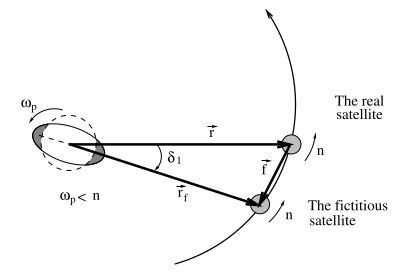
\includegraphics[scale=.8]{Image/shema_planete.png}
	\end{center}
	
	Ici nous nous intéresseront aux astres à \textbf{faible excentricité} et évoluant \textbf{près de l'équateur} (orbite équatoriale et circulaire).\\
	
	Ce qui est le cas de Phobos par rapport à Mars.
	
	\subsection{Effet de marée}
	
	Le cœur de l'article \cite{etude} était d'améliorer la modélisation des effets de marées entre une planète et l'un de ses satellites (une application numérique a été faite pour Phobos, une lune de Mars).\\

    On se place dans la cadre simplifié de l’article, en supposant l'orbite de Phobos circulaire et équatorial pour pouvoir se mettre dans l'approximation des petits angles notamment.

   Le cœur du phénomène de marée provient du décalage entre la position du satellite et la réponse déformée de la planète. En effet, l’attraction gravitationnelle d’un satellite déforme la planète et crée une bosse de marée. Or, le manteau planétaire étant viscoélastique, cette déformation ne se produit pas instantanément mais avec un certain retard. Cette déformation modifie alors le champ gravitationnel exercé par la planète sur le satellite.

    Si la bosse se forme en avant du satellite, c'est à dire que la planète tourne plus rapidement sur elle-même que le satellite n'orbite autour d'elle, cette bosse va accélérer le satellite dans le sens de son mouvement et celui-ci va s'échapper de l'orbite à terme (comme la Lune avec la Terre).

    Dans le cas contraire, si la bosse est située en arrière du satellite, elle le freine. Il va alors finir par chuter sur la planète comme c'est le cas ici de Phobos.

    Pour modéliser ce phénomène, introduisons les grandeurs suivantes ( A MODIFIER POUR BONNE REFERENCE voir schéma issu de l'article). Le satellite situé à la position planétocentrée $\mathbf r$ déforme donc la planète avec un retard $\Delta t$ et un décalage spatial $\mathbf f$ qui correspond à la position d'un satellite fictif par rapport au satellite si la déformation était instantanée. L'angle de retard entre la position réelle du satellite et la position du satellite fictif est noté $\delta$. Nous avons donc avec  $\mathbf r_f$ la position panétocentrée  : 
    \[
\mathbf r_f=\mathbf r+\mathbf f,
\qquad
\mathbf f=\Delta t(\boldsymbol{\omega}_p\times\mathbf r-\mathbf v).
\]
    Où $\omega_p$ désigne la vitesse de rotation de la planète et $n$ la fréquence orbitale moyenne du satellite, c’est-à-dire sa vitesse angulaire de révolution autour de la planète.

    On introduit également la fréquence principale des marées $\chi$. Notons que les marées se produisent deux fois par révolution du satellite. En effet, une seconde bosse de marée se forme également du côté opposé au satellite. C’est pour cette raison que sur Terre les marées hautes dues à la Lune ont lieu environ toutes les $12\,h\,25$, alors que la Terre tourne sur elle-même en $24\,h$ et que la Lune effectue une révolution autour de la Terre en  $27$ jours.

    Toutes ces grandeurs sont liées par les relations suivantes dans l’approximation des petits angles. En supposant le triangle formé par $\mathbf r$ et $\mathbf f$ localement rectangle, on obtient :

\[
\delta \approx \frac{|\mathbf f|}{r}
=
\frac{\Delta t}{2}\chi,
\qquad
\chi = 2|\omega_p-n|,
\]

où $\omega_p$ désigne la vitesse de rotation de la planète et $n$ la fréquence orbitale moyenne du satellite, c’est-à-dire sa vitesse angulaire de révolution autour de la planète.
     
    Cette relation est fondamentale pour la suite car elle relie la géométrie du décalage  de marée à la dynamique orbitale du système. En effet, le retard angulaire $\delta$ dépend donc de la fréquence de marée $\chi$ qui est deux fois la différence entre la vitesse de rotation de la planète et de révolution du satellite. Dans la suite, nous verrons également comment ce phénomène est lié à la dissipation d’énergie dans le manteau en introduisant le facteur de qualité $Q$ ainsi que sa relation avec  $\delta$. L’objectif principal de l’article est précisément d’étudier comment cette dissipation dépend de la fréquence des marées et comment cela modifie l’évolution orbitale du satellite.

NOUVEAU TITRE FACTEUR DE QUALIT2 Q 

    La réponse viscoélastique interne du manteau aux forces de marée est un phénomène extrêmement complexe faisant intervenir de nombreux mécanismes (dislocations, la diffusion de défauts ponctuels ou encore les interactions entre joints de grains). plutôt que de modéliser l'ensemble de ces phénomènes directement, les planétologues introduisent le paramètre $Q$ ou facteur de qualité qui mesure le taux de dissipation d'énergie dans le manteau de façon analogue au facteur d'amortissement dans l'équation d'un oscillateur harmonique amorti. 

    Le facteur de qualité $Q$ dépend de la fréquence $\chi$. D’anciens modèles de marée cités dans l'article supposaient soit un facteur de qualité constant, soit une loi en :

\[
Q \sim \chi^{-1}.
\]

Cependant, des mesures expérimentales en laboratoire à basse fréquence ainsi que des observations sismologiques ont progressivement mis en évidence une loi plus réaliste :

\[
Q \sim \chi^\alpha.
\]

Dans la plage de fréquences suivantes 

\[
1\,an^{-1} \lesssim \chi \lesssim 10^7 \text{ Hz},
\]

les mesures donnent généralement :

\[
0.2 \leq \alpha \leq 0.4.
\]

Cette plage étant très large, elle englobe évidemment la fréquence du phénomène de marée entre Mars et Phobos. 

Cette loi montre que plus la fréquence du phénomène de marée augmente, plus le facteur de qualité $Q$ augmente, soit l'énergie dissipée diminue. Ainsi à haute fréquence c'est le caractère élastique du manteau qui domine face au comportement visqueux car cette réponse visqueuse est très lente.

L’article montre également, par un calcul énergétique et dans l’approximation des petits angles, que :

\[
Q^{-1}\approx 2\delta.
\]

Ainsi, lorsque $Q$ augmente, le retard angulaire $\delta$ diminue, ce qui est cohérent avec une dissipation plus faible.

En reprenant la relation :

\[
\delta \approx \frac{\Delta t}{2}\chi,
\]

on obtient :

\[
\Delta t = \mathcal{E}^\alpha \chi^{-(\alpha+1)}
=
\mathcal{E}^\alpha \left(2|\omega_p-n|\right)^{-(\alpha+1)}.
\]

Où le paramètre $\mathcal{E}$ est un facteur dimensionné homogène à un temps permettant de conserver l'homogénéité Il peut être interprété comme un temps de relaxation de la dissipation dans le manteau. 

Ainsi, On obtient des liens étroits entre le retard des marées, la fréquence du phénomène et l’énergie dissipée dans le manteau planétaire. Ce couplage  est au coeur du modèle de l'artilce pour décrire l'évolution de l'orbite de Phobos. 

    
TITRE OBTENTION DE L'EQUATION SUR LE DEMI GRAND AXE DE PHOBOS

L’article établit ensuite l’équation du mouvement du satellite :

\[
\ddot{\mathbf r}
=
-\frac{G(M_0+m)}{r^3}\mathbf r
+
\mathbf F_{\text{marée}}.
\]

Le premier terme correspond à l’attraction gravitationnelle classique du problème à deux corps. Le terme $\mathbf F_{\text{marée}}$ désigne quant à lui la force supplémentaire résultant du potentiel de marée agissant sur le satellite, i.e. l’attraction gravitationnelle exercée par la bosse de marée de la planète sur le satellite. On étudie donc ici l’effet de la déformation de la planète sur le satellite qui a lui-même généré cette déformation. L'articule tronque le développement du potentiel de marée au terme dominant correspondant à la déformation quadrupolaire. On obtient alors la force des marées :

\[
\mathbf F_{\text{marée}}
=
-\frac{3k_2G(M_0+m)mR^5}{r^{10}M_0}
\left[
\mathbf -f\,r^2
-
2\mathbf r(\mathbf r\cdot\mathbf f)
\right].
\]

avec :
\begin{itemize}
    \item $k_2$ : le nombre de Love quadrupolaire ;
    \item $R$ : le rayon de la planète ;
    \item $M_0$ : la masse de la planète ;
    \item $m$ : la masse du satellite ;
    \item $\mathbf f$ : le retard spatial de la bosse de marée.
\end{itemize}


    La dernière étape pour obtenir l’évolution du demi-grand axe orbital de Phobos consiste à projeter cette force sur la composante tangentielle du mouvement du satellite. En effet, c’est cette composante tangentielle de la force de marée qui est responsable des échanges d’énergie et donc de l’évolution du demi-grand axe. 


    On obtient alors l’équation suivante, que l’on résoudra numériquement dans la suite :

\[
\frac{da}{dt}
=
\frac{6k_2R^5nm\Delta t}{M_0a^4}(n-\omega_p),
\]

avec pour rappel :

\[
\Delta t
=
\mathcal{E}^{\alpha}
\left(2|n-\omega_p|\right)^{-(\alpha+1)}.
\]
	
	\subsection{Approximations}
	
	\subsubsection{Limite de Roche}
	
	\subsection{Équation sur le demie-grand axe}

    
    
	
	
\end{document}